\subsubsection{Measurements using $H \to \gamma\gamma$, $H \to ZZ^* \to 4\ell$, (boosted) \Hbb decay channels}
\label{sec:diffxs}

\begin{center}{\it Written by: T. Klijnsma} \end{center}

% Assuming the following concepts are already defined (if not, should be defined here):
% HL-LHC, pT_H, SM, S1, S2

\todo{This section now closely follows FTR-18-011, and describes only CMS results.}

In the context of Higgs boson property measurements, one of the main goals of HL-LHC, differential measurements provide a probe of various Higgs boson properties by looking at distortions of differential distributions.
% 
The $\pTH$ distribution is of particular interest, as potential new physics may reside in the tails of the distribution, which cannot be measured in inclusive measurements~\cite{%
Khachatryan:2016vau,% 7 & 8 TeV coupling combination
Aad:2015zhl,% 7 & 8 TeV mass combination
CMS:2018lkl% 13 TeV CMS coupling combination
}.
% 
Differential Higgs boson production cross section measurements are available for a range of observables from both the ATLAS~\cite{%
Aad:2014lwa,% diff. ATLAS hgg, Run I
Aad:2014tca,% diff. ATLAS hzz, Run I
Aad:2016lvc,% diff. ATLAS hww, Run I
Aaboud:2018xdt,% diff. ATLAS hgg, Run II
Aaboud:2017oem,% diff. ATLAS hzz, Run II
Aaboud:2018ezd% diff. ATLAS combination Run II    
} and CMS~\cite{%
Khachatryan:2015rxa,% diff. CMS hgg, Run I
Khachatryan:2015yvw,% diff. CMS hzz, Run I
Khachatryan:2016vnn,% diff. CMS hww, Run I
Sirunyan:2018kta,% diff. CMS hgg, Run II
CMS_AN_2016-442,% diff. CMS hzz, Run II
CMS-PAS-HIG-17-028% diff. CMS combination Run II
} Collaborations at $\sqrt{s}=8$ and $13$\UTeV.
% 
The most recent $\pTH$ spectra at $\sqrt{s}=13$\UTeV from both the ATLAS~\cite{Aaboud:2018ezd} and CMS~\cite{CMS-PAS-HIG-17-028} Collaborations are projected to an integrated luminosity of $3000\fbinv$.
% 
The projection of the $\pTH$ spectrum at $3000\fbinv$ by the CMS Collaboration is shown in Fig.~\ref{fig:proj_pth}, for both S1 and S2.
% 
The corresponding relative uncertainties for both scenarios are given in Tables~\ref{tab:proj_pth_unc_scen1} and \ref{tab:proj_pth_unc_scen2}.
% 
With respect to the uncertainties at the current integrated luminosity of 35.9\fbinv, the uncertainties at 3000\fbinv in the higher $\pTH$ region are about a factor of ten smaller. This is expected, as the uncertainties in this region remain statistically dominated.
% 
The uncertainties in the lower $\pTH$ region are no longer statistically dominated however, as can been seen by comparing Table~\ref{tab:proj_pth_unc_scen1} with Table~\ref{tab:proj_pth_unc_scen2}, where the reduced systematic uncertainties in S2 yield a reduction in the total uncertainty of up to 25\% compared to S1.


\begin{figure}[hbtp]
  \begin{center}
    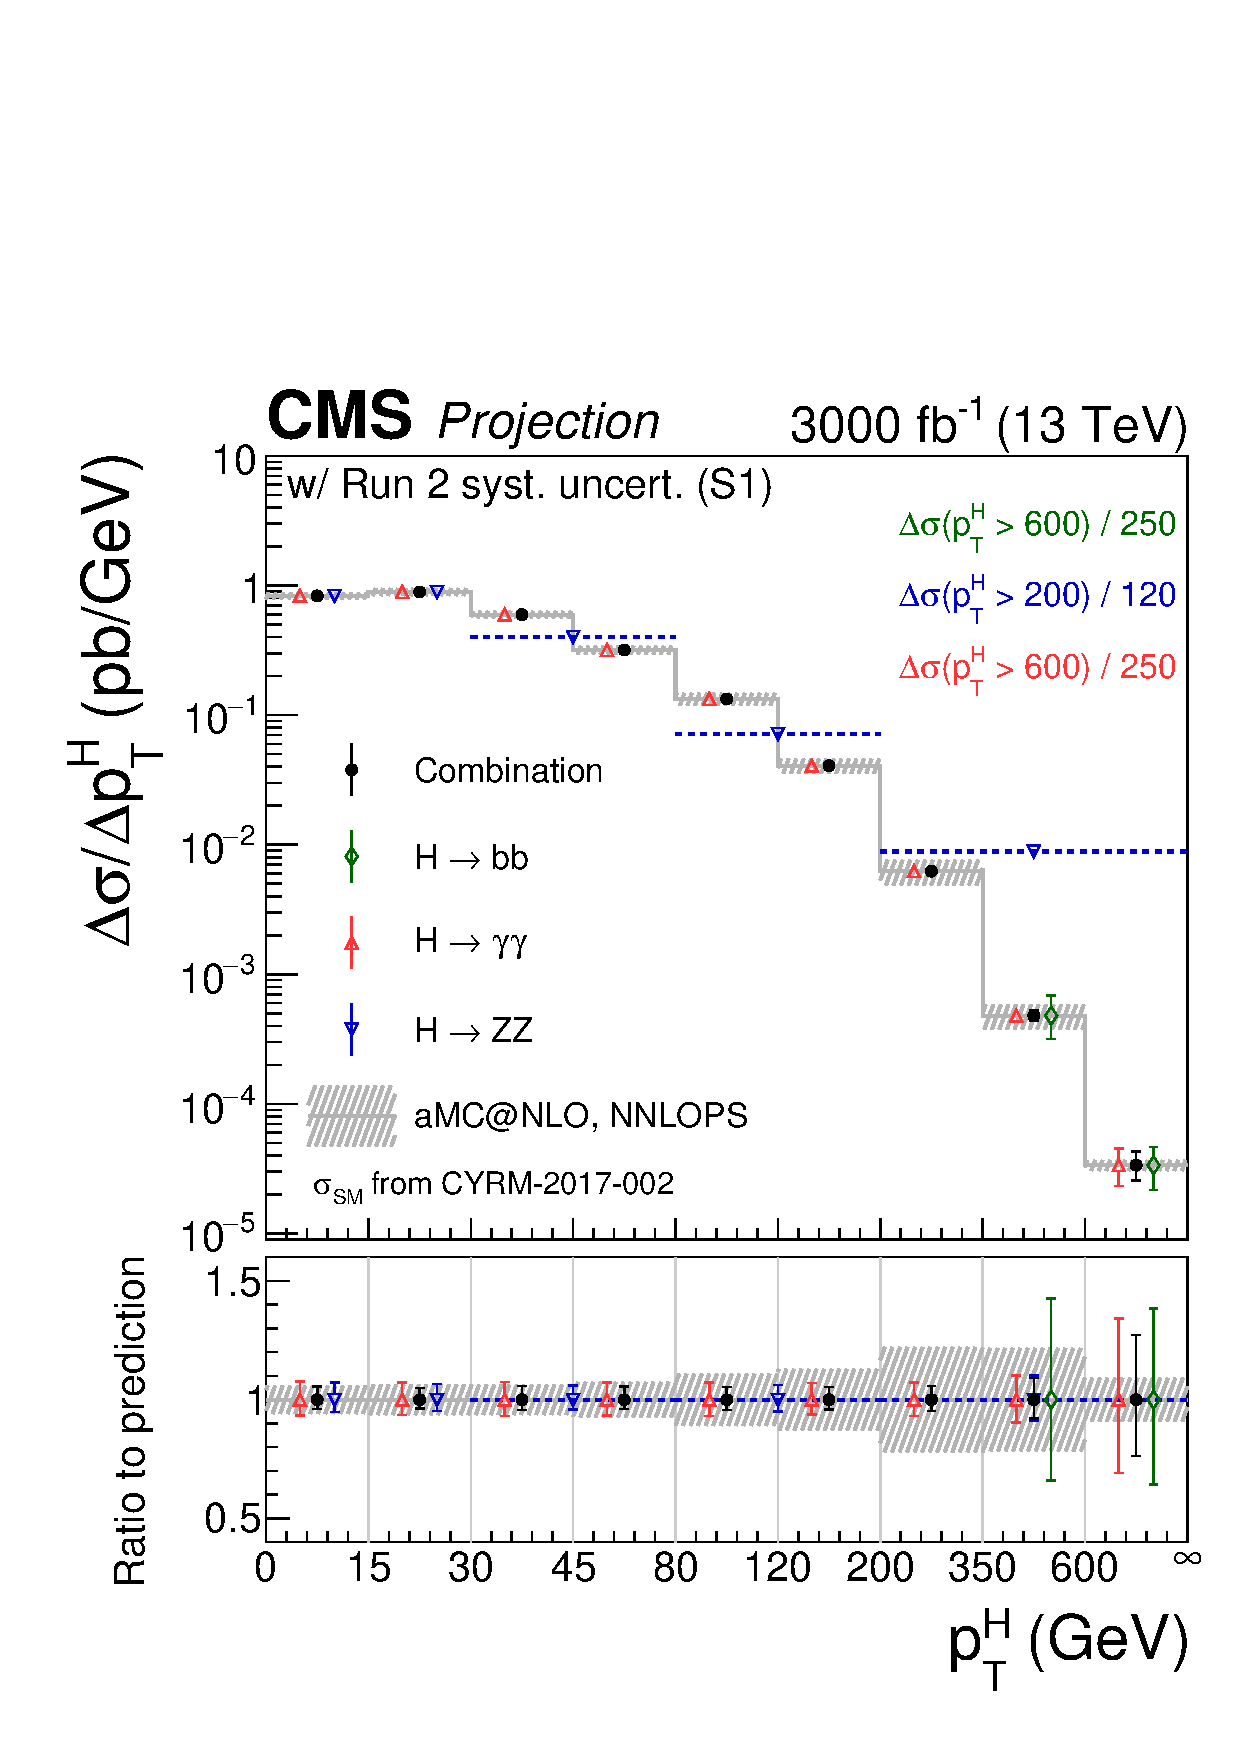
\includegraphics[width=0.49\linewidth]{\main/section2/plots/differentials/projectionspectra_pth_smH.pdf}
    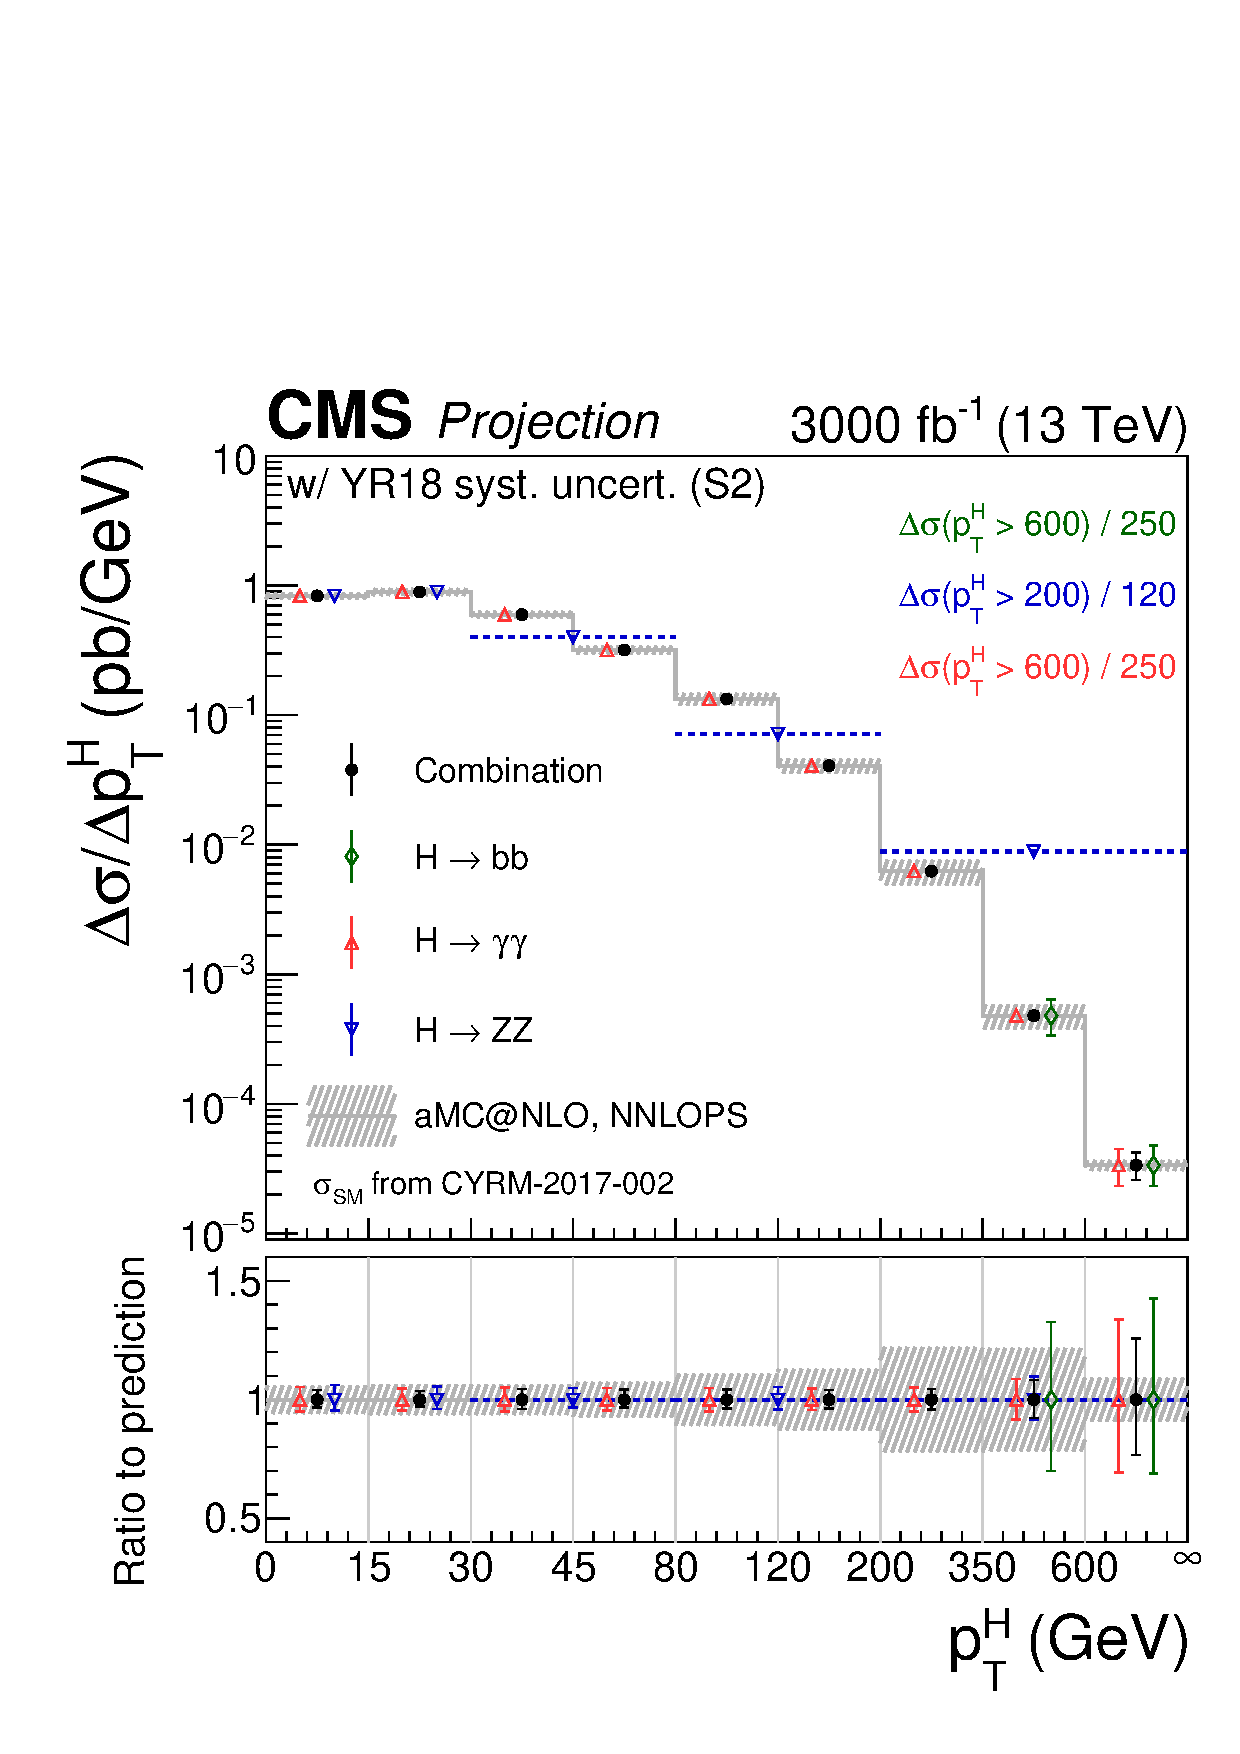
\includegraphics[width=0.49\linewidth]{\main/section2/plots/differentials/projectionspectra_pth_smH_scenario2.pdf}
    \caption{
        Projected differential cross section for the $\pTH$ spectrum at an integrated luminosity of 3000\fbinv, under S1 (\UcmsLeft, with Run~2 systematic uncertainties~\cite{CMS-PAS-HIG-17-028}) and S2 (\UcmsRight, with YR18 systematic uncertainties).
        }
    \label{fig:proj_pth}
  \end{center}
\end{figure}

\begin{table}[htb]
\footnotesize
\begin{center}
\begin{tabular}{l|c|c|c|c|c|c|c|c|c}
% \hline
$\pTH$ (GeV)       & 0-15    &  15-30   &  30-45    &  45-80   &  80-120  &  120-200  &  200-350  &  350-600  &  600-$\infty$  \\
\hline
$\hgg$       & $7.2\%$ & $6.8\%$ & $7.1\%$ & $6.9\%$            & $7.1\%$ & $6.7\%$            & $7.1\%$ & $9.9\%$  & $32.5\%$ \\ 
% \hline 
$\hzz$       & $6.2\%$ & $5.7\%$ & \multicolumn{2}{c|}{$5.0\%$} & \multicolumn{2}{c|}{$5.5\%$} & \multicolumn{3}{c}{$9.6\%$} \\ 
% \hline 
$\hbb$       & \multicolumn{7}{c|}{\textit{None}}                                              & $38.2\%$ & $37.1\%$ \\ 
% \hline 
Combination  & $4.7\%$ & $4.4\%$ & $5.0\%$ & $4.7\%$            & $4.8\%$ & $4.7\%$            & $5.2\%$ & $8.5\%$  & $25.4\%$ \\
% \hline
\end{tabular}
\end{center}
\caption{
    Relative uncertainties on the projected $\pTH$ spectrum under S1 (with Run~2 systematic uncertainties~\cite{CMS-PAS-HIG-17-028}) at $3000\fbinv$.
    }
\label{tab:proj_pth_unc_scen1}
\end{table}

\begin{table}[htb]
\footnotesize
\begin{center}
\begin{tabular}{l|c|c|c|c|c|c|c|c|c}
% \hline
$\pTH$ (GeV)       & 0-15    &  15-30   &  30-45    &  45-80   &  80-120  &  120-200  &  200-350  &  350-600  &  600-$\infty$  \\
\hline
$\hgg$       & $5.1\%$ & $4.6\%$ & $5.1\%$ & $4.8\%$            & $4.9\%$ & $4.5\%$            & $5.1\%$ & $8.6\%$  & $32.2\%$ \\ 
% \hline 
$\hzz$       & $5.4\%$ & $4.8\%$ & \multicolumn{2}{c|}{$4.1\%$} & \multicolumn{2}{c|}{$4.7\%$} & \multicolumn{3}{c}{$9.1\%$} \\ 
% \hline 
$\hbb$       & \multicolumn{7}{c|}{\textit{None}}                                              & $31.4\%$ & $36.8\%$ \\ 
% \hline 
Combination  & $3.7\%$ & $3.3\%$ & $4.2\%$ & $3.7\%$            & $4.0\%$ & $3.8\%$            & $4.4\%$ & $8.0\%$  & $24.5\%$ \\
% \hline
\end{tabular}
\end{center}
\caption{
    Relative uncertainties on the projected $\pTH$ spectrum under S2 (with YR18 systematic uncertainties) at $3000\fbinv$.
    }
\label{tab:proj_pth_unc_scen2}
\end{table}


Due to a different choice of binning and the lack of a more sophisticated study of the correlation of systematic uncertainties, it was chosen not to combine the presented projected spectra from the ATLAS and CMS Collaborations.
% 
Instead, the projections from CMS are scaled to an integrated luminosity of 6000\fbinv, providing an estimate of the overall sensitivity of an eventual combination of the two experiments.
% 
Figure~\ref{fig:proj_pth_6000} shows the CMS projection at 6000\fbinv, with the same systematic scaling as for the projection at 3000\fbinv.
% 
As expected at very high integrated luminosity, the systematic uncertainties dominate the statistical ones.


\begin{figure}[hbtp]
  \begin{center}
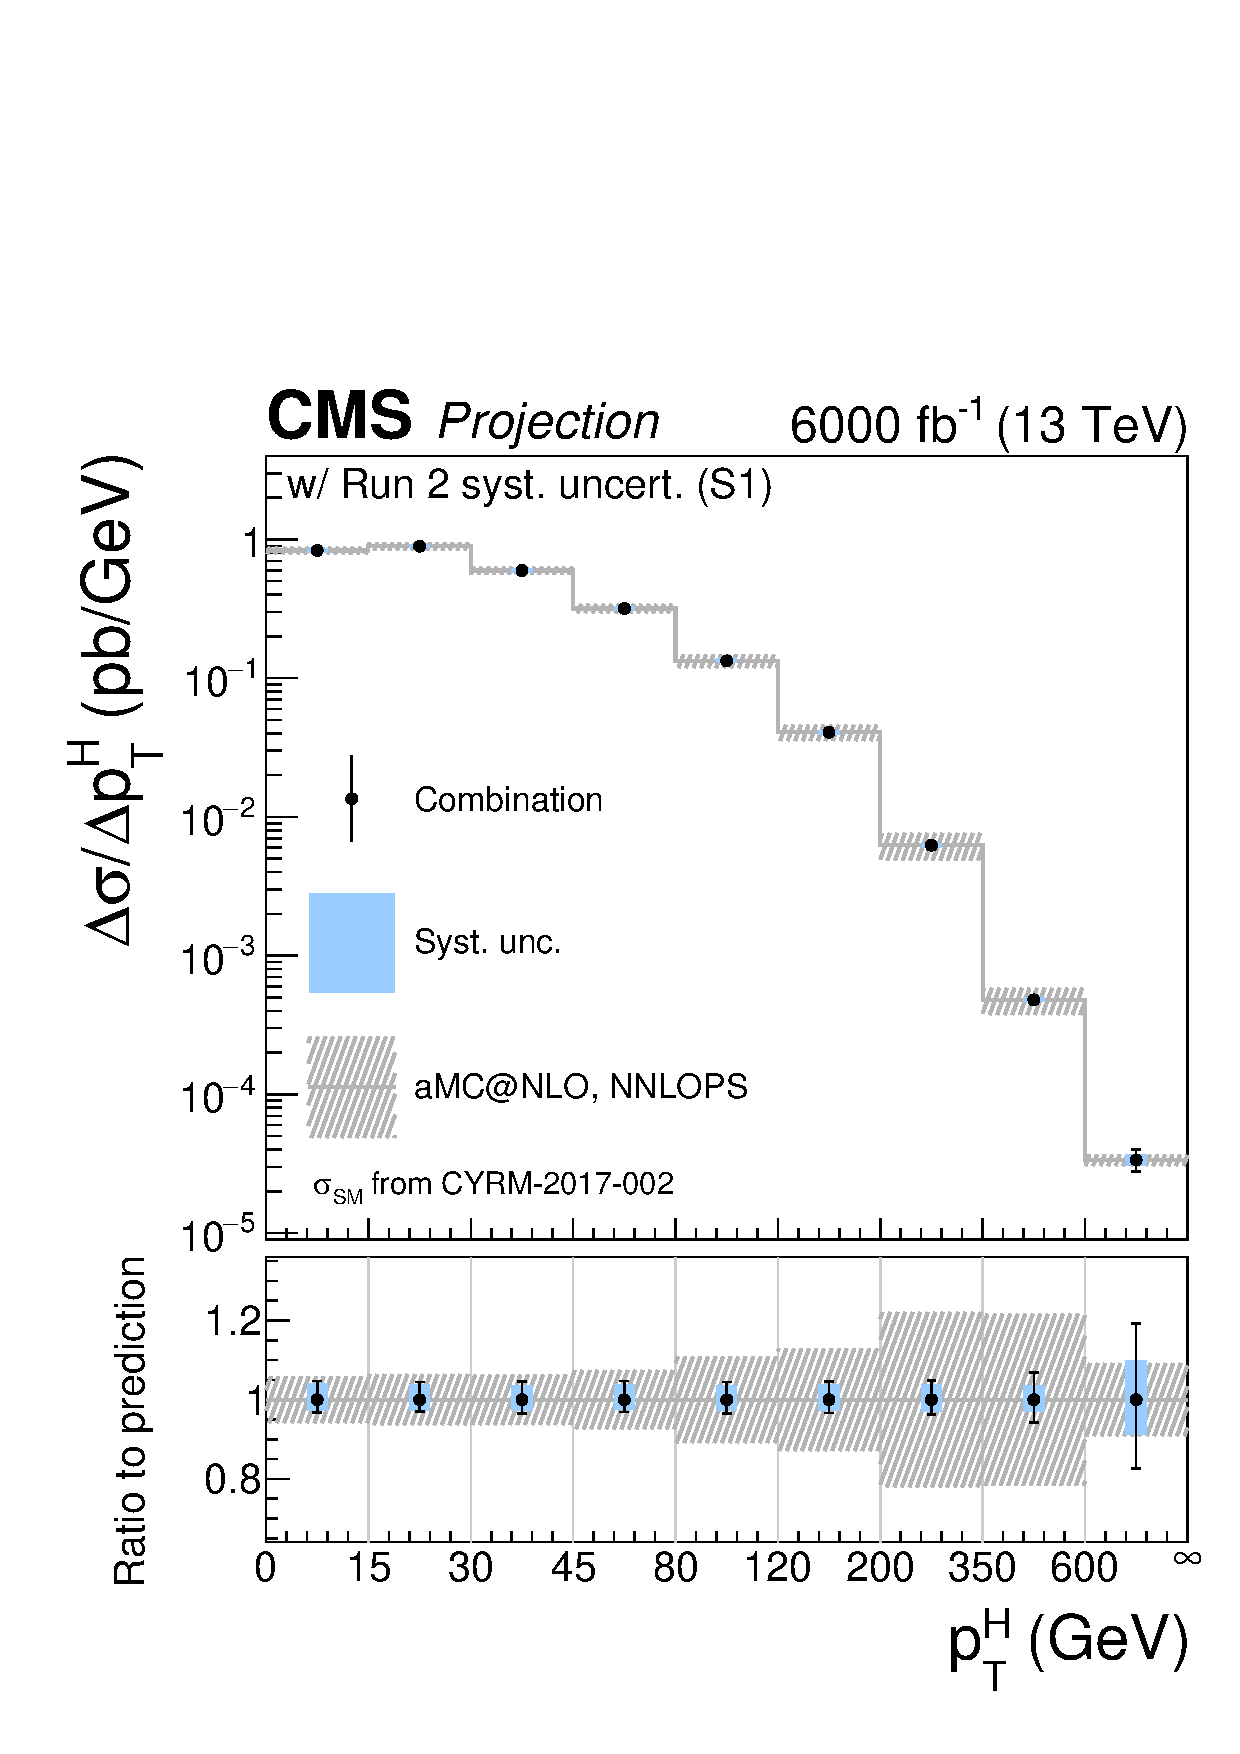
\includegraphics[width=0.49\linewidth]{\main/section2/plots/differentials/projectionspectra_pth_smH_lumi6000.pdf}
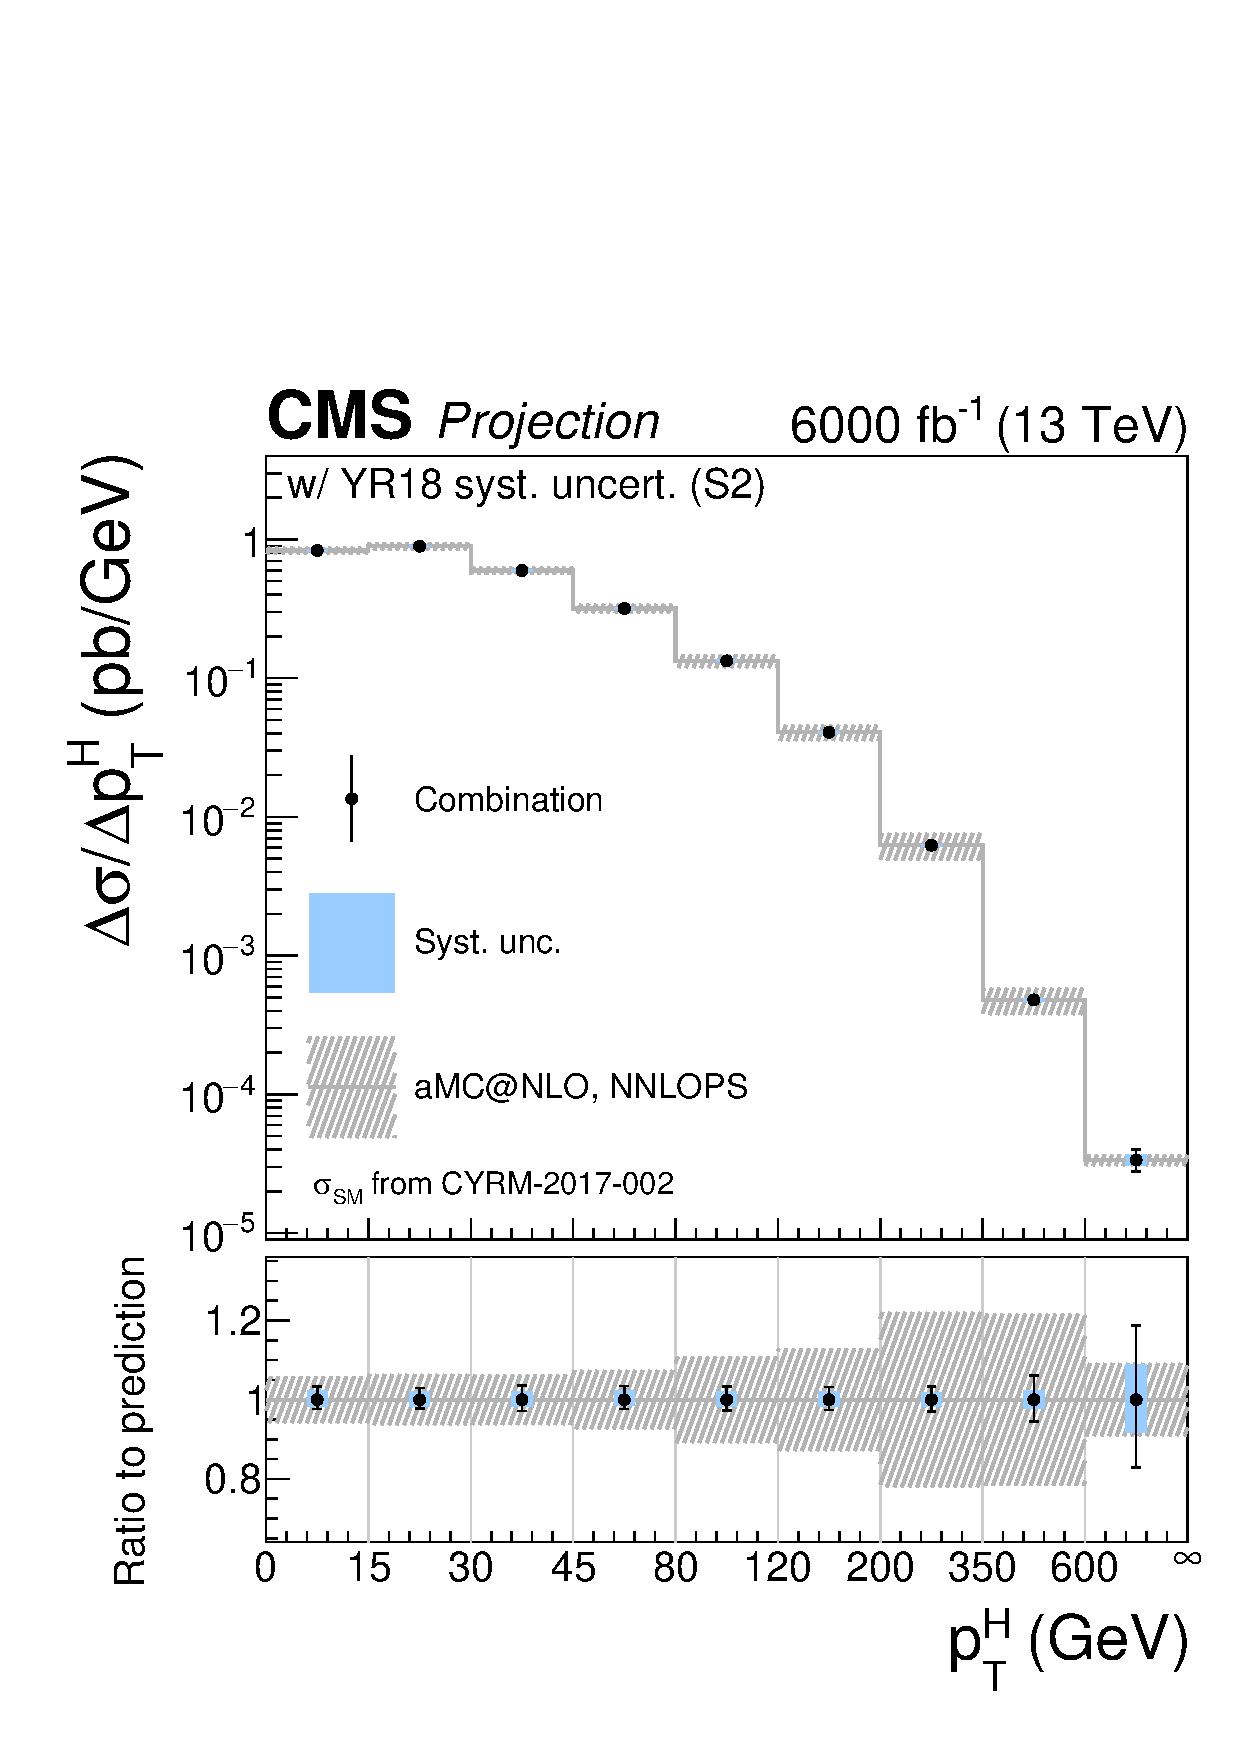
\includegraphics[width=0.49\linewidth]{\main/section2/plots/differentials/projectionspectra_pth_smH_lumi6000_scenario2.pdf}
    \caption{
        Projected differential cross section for the $\pTH$ spectrum at an integrated luminosity of 6000\fbinv (representing the sensitivity achievable by an eventual ATLAS and CMS combination), under S1 (\UcmsLeft, with Run~2 systematic uncertainties~\cite{CMS-PAS-HIG-17-028}) and S2 (\UcmsRight, with YR18 systematic uncertainties).
        }
    \label{fig:proj_pth_6000}
  \end{center}
\end{figure}

%------------------------ End differentials


\subsubsection{Measurement of $p_{T}(H)$ spectrum  in \ttH production mode}
\begin{center}{\it To be written by: N. Wardle} \end{center}
